\subsection{L'implémentation des anti-windups}
\label{sec:anti_windup}

Dans un contrôleur PID, le terme de l'intégral a pour rôle d'éliminer l'erreur statique en accumulant l'erreur au cours du temps. Cependant, lorsque l'actionneur atteint ses limites physiques de fonctionnement, la commande calculée par le contrôleur ne peut plus être appliquée intégralement. On parle alors de saturation de l'actionneur. \\

Dans cette situation, le terme intégral continue d'accumuler l'erreur alors même que l'actionneur est incapable de produire une commande supplémentaire. Ce phénomène est appelé saturation de l'intégrateur. Lorsque le système quitte la saturation, l'intégrateur contient une valeur excessive qui continue d'influencer la commande pendant un certain temps. Cela peut entraîner un dépassement important de la consigne, des oscillations ainsi qu'une augmentation du temps de stabilisation du système. (cf. figure \ref{fig:integralWindup}) \\

L'objectif d'un anti-windup est d'empêcher ou de limiter cette accumulation excessive du terme intégral pendant les phases de saturation. En réduisant l'effet windup, le contrôleur retrouve plus rapidement un fonctionnement normal lorsque la saturation disparaît. Les performances dynamiques du système sont ainsi améliorées, notamment par une diminution du dépassement, une réduction du temps de réponse et une meilleure stabilité globale. \\

Le principe général d'un anti-windup consiste à modifier le calcul du terme intégral lorsque la commande est saturée. Plusieurs approches existent, parmi lesquelles les plus répandues sont :
\begin{itemize}
    \item \textbf{l'anti-windup clamp}, qui bloque ou limite directement la valeur du terme intégral lorsque 
    celui-ci atteint une borne prédéfinie
    \item \textbf{l'anti-windup back-calculation}, qui corrige progressivement l'intégrateur en fonction de 
    l'écart entre la commande calculée par le PID et la commande réellement appliquée après la saturation
\end{itemize}

\begin{figure}
    \centering
    
\includegraphics[width=\textwidth]{images/integralWindup.png}
    \caption{Principe de l'anti-windup sur l'intégral du PID}
    \label{fig:integralWindup}
\end{figure}

\subsubsection{L'anti-windup clamp}
\label{sec:anti_windup_clamp}

L'anti-windup clamp consiste à limiter la valeur du terme intégral à une certaine plage. Lorsque la commande calculée par le PID dépasse les limites de l'actionneur, le terme intégral est "clampé" à une valeur maximale ou minimale prédéfinie. Cela empêche l'intégrateur de continuer à accumuler l'erreur et de provoquer un dépassement excessif lorsque la saturation disparaît. \\

Le terme intégral est calculé comme suit :
\begin{equation}
    I_{k} = I_{k-1} + K_i e_{k} \Delta t
\end{equation}

où :
\begin{itemize}
    \item $I_{k}$ est la valeur du terme intégral à l'instant $k$
    \item $K_i$ est le gain intégral du PID
    \item $e_{k}$ est l'erreur à l'instant $k$
    \item $\Delta t$ est le pas de temps de l'échantillonnage
\end{itemize}

Après la saturation de l'actionneur, le terme intégral est limité à une valeur maximale ou minimale prédéfinie :
\begin{equation}
    I_{k} =
    \begin{cases}
        I_{max}, & \text{si } I_{k} > I_{max} \\
        I_{min}, & \text{si } I_{k} < I_{min} \\
        I_{k}, & \text{sinon}
    \end{cases}
\end{equation}

\paragraph{Avantages}

L'anti-windup clamp présente plusieurs avantages :
\begin{itemize}
    \item Il est simple à implémenter et à configurer
    \item Il permet de limiter rapidement l'accumulation du terme intégral lors de la saturation
    \item Il améliore la stabilité du système en évitant les dépassements excessifs
\end{itemize}

\paragraph{Inconvénients}

Il présente également quelques inconvénients :
\begin{itemize}
    \item Il peut introduire des discontinuités dans la commande, ce qui peut provoquer des oscillations ou des 
    comportements indésirables
    \item Il nécessite de définir des bornes appropriées pour le terme intégral, ce qui peut être difficile dans 
    certains systèmes
    \item Il peut ne pas être efficace dans les systèmes avec des dynamiques complexes ou des non-linéarités 
    importantes
\end{itemize}

\subsubsection{L'anti-windup back-calculation}
\label{sec:anti_windup_back_calculation}

L'anti-windup back-calculation est une approche plus élaborée qui ne consiste pas à limiter l'intégrateur directement, mais à chercher à le corriger afin qu'il reflète la commande effectivement appliquée au système.

Soit :
\begin{itemize}
    \item $u$ la commande calculée par le PID
    \item $u_{sat}$ la commande après saturation
\end{itemize}

La différence $u_{sat} - u$ représente l'erreur introduite par la saturation. Le principe de back-calculation consiste à réinjecter cette erreur dans l'intégrateur :
\begin{equation}
    I_{k} = I_{k-1} + K_i e_{k} \Delta t + K_{aw} (u_{sat_k} - u_{k})
\end{equation}

où :
\begin{itemize}
    \item $K_{aw}$ est le gain de l'anti-windup
    \item $u_{k}$ est la commande calculée
    \item $u_{sat_k}$ est la commande réellement envoyée à l'actionneur
\end{itemize}

Lorsque le contrôleur est saturé, la différence ($u_{sat}- u$) devient importante. Le terme correcteur agit alors sur l'intégrateur afin de réduire progressivement son accumulation ; Dès que le système quitte la saturation, l'intégrateur possède déjà une valeur proche de celle nécessaire au fonctionnement normal du contrôleur. \\

Le paramètre essentiel de cette méthode est le gain $K_{aw}$. Un gain trop faible rend la correction peu efficace, tandis qu'un gain trop élevé peut introduire des oscillations ou dégrader la stabilité du système. En pratique, il est souvent choisi sous la forme :
\begin{equation}
    K_{aw} = \frac{1}{T_{t}}
\end{equation}

où $T_{t}$ est une constante de temps d'anti-windup réglée en fonction de la dynamique du système. \\

\paragraph{Avantages}

Il présente plusieurs avantages :
\begin{itemize}
    \item Il possède une récupération rapide après une saturation
    \item Il réduit fortement le dépassement
    \item Il est plus fidèle au comportement réel de l'actionneur
\end{itemize}

\paragraph{Inconvénients}

Il présente également quelques inconvénients :
\begin{itemize}
    \item Il est plus complexe à implémenter et à configurer
    \item Il nécessite un réglage précis du gain $K_{aw}$ pour éviter les oscillations ou la dégradation de la stabilité
    \item Il peut être sensible aux variations de la dynamique du système ou aux perturbations externes
\end{itemize}

\subsubsection{Illustration par un cas pratique}
\label{sec:illustration_drone}

\RemarkBox
{Point important}
{
Dans cette section, il faut bien comprendre que tout est dans un contexte de simulation, et que les résultats obtenus ne sont pas forcément représentatifs de la réalité. Cette section a pour but de montrer l'impact de l'anti-windup sur un système de contrôle, et non pas de fournir une solution optimale pour le contrôle d'un drone.
}

Pour tester l'efficacité de l'anti-windup, nous avons choisi un cas pratique simple mais représentatif : le contrôle d'altitude d'un drone en fonction de la vitesse de rotation de ses hélices, en suivant l'exemple donné dans la vidéo \href{https://www.youtube.com/watch?v=NVLXCwc8HzM&list=PLn8PRpmsu08pQBgjxYFXSsODEF3Jqmm-y&index=24}{Anti-windup for PID control | Understanding PID Control, Part 2}. L'objectif est de maintenir le drone à une altitude cible en ajustant la vitesse de rotation des hélices. \\

Pour réussir cela, nous avons mis en place un contrôleur PID qui calcule la commande à envoyer aux hélices en fonction de l'erreur entre l'altitude cible et l'altitude actuelle du drone. Cependant, la vitesse de rotation des hélices est limitée à 15 tours/minute, ce qui peut entraîner une saturation de la commande lorsque le drone est loin de l'altitude cible. Dans ce cas, l'intégrateur du PID peut continuer à accumuler l'erreur, ce qui peut provoquer un dépassement important de l'altitude cible lorsque le drone quitte la saturation. \\

Dans notre scénario, nous avons simulé une situation où le drone est initialement à une altitude de 0 mètre et doit atteindre une altitude cible de 5 mètres. Cependant, nous avons introduit une retenue de 10 secondes avant que le drone ne commence à monter, ce qui provoque une accumulation importante de l'erreur dans l'intégrateur du PID. \\

Nous avons donc mis en place deux types d'anti-windup : le clamp et le back-calculation, afin de comparer leurs performances dans ce scénario.

\subsubsection{La configuration du système de contrôle}
\label{sec:configuration_drone}

\begin{figure}
    \centering
    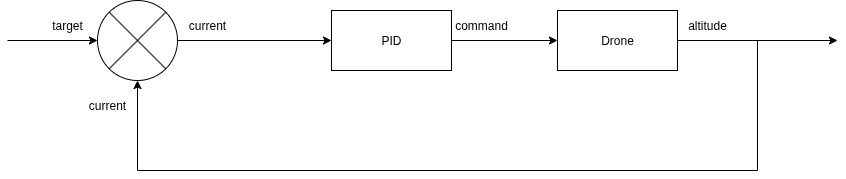
\includegraphics[width=\textwidth]{images/schéma_bloc_fonctionel_drone.png}
    \caption{Schéma bloc fonctionnel du système de contrôle du drone}
    \label{fig:schéma_bloc_fonctionel_drone}
\end{figure}

Le système de contrôle est composé d'un contrôleur PID qui reçoit en entrée l'erreur entre l'altitude cible et l'altitude actuelle du drone, et qui calcule la commande à envoyer aux hélices pour corriger cette erreur. Le contrôleur PID est configuré avec les paramètres suivants : 

\begin{equation}
K_p = 1{.}5, \quad K_i = 0{.}6, \quad K_d = 0
\end{equation}

Le système est simulé avec un pas de temps de 0.1s, et l'altitude cible est fixée à 5 mètres. Le drone est initialement à une altitude de 0 mètre, et la vitesse de rotation des hélices est limitée à 15 tours/minute. \\

Le drone est modélisé par les équations suivantes :
\begin{equation}
\begin{cases}
    a = \frac{F_{p}}{m} - g - \frac{C_{d}v}{m} \\
    v(t + \Delta t) = v(t) + a \Delta t \\
    h(t + \Delta t) = h(t) + v \Delta t
\end{cases}
\end{equation}

Où : 
\begin{itemize}
    \item $a$ est l'accélération verticale du drone (m/s²)
    \item $F_{p}$ est la force de poussée générée par les hélices (N)
    \item $m$ est la masse du drone (kg)
    \item $g$ est l'accélération gravitationnelle (m/s²)
    \item $C_{d}$ est le coefficient de frottement de l'air
    \item $v$ est la vitesse verticale du drone (m/s)
    \item $h$ est l'altitude du drone (m)
    \item $\Delta t$ est le pas de temps de la simulation (s) 
\end{itemize}

La force de poussée générée par les hélices est calculée par l'équation suivante :
\begin{equation}
F_{p} = 4 * KP * (\frac{2 \pi}{60})^{2} * u^{2}
\end{equation}

Où :
\begin{itemize}
    \item $KP$ est la constante de poussée d'une hélice
    \item $u$ est la vitesse de rotation des hélices (tour/min)
\end{itemize}

Parmi les constantes physiques du drone qui sont paramétrées comme ceci :
\begin{equation}
    m = 0{.}2, \quad g = 9{.}81, \quad KP = 0.29, \quad C_{d} = 0{.}8
\end{equation}

Pour la configuration de l'anti-windup clamp, nous avons choisi de limiter le terme intégral à une valeur maximale de 30 et une valeur minimale de -30. \\

Pour la configuration de l'anti-windup back-calculation, nous avons choisi un gain $K_{aw} = \frac{1}{0.2}$

\subsubsection{Evaluation des performances}
\label{sec:evaluation_perf_anti_windup}

Pour évaluer les performances du système de contrôle avec et sans anti-windup, nous avons simulé le même scénario dans des conditions parfaites, c'est-à-dire sans la retenue de 10 secondes. Pour qu'on puisse se rendre compte des performances des anti-windups dans ces conditions. \\

Parmi les critères d'évaluation, nous avons choisi de mesurer l'altitude maximale atteinte par le drone, le dépassement maximal de l'altitude cible\footnote{Signifie le pourcentage que représente l'écart entre l'altitude atteinte et l'altitude cible par rapport à l'altitude cible}, le temps de stabilisation du système, l'intégrale maximale de l'erreur et les commandes maximales, minimales et moyennes envoyées aux hélices. \\

Avec ces critères d'évaluation, nous avons pu comparer les performances du système de contrôle avec et sans anti-windup, et ainsi déterminer l'impact de l'anti-windup sur le comportement du drone. \\

Les critères d'évaluation les plus pertinents sont le dépassement maximal de l'altitude cible et la stabilisation du drone. On peut observer que l'anti-windup permet de réduire le dépassement maximal de l'altitude cible drastiquement. En effet, sans anti-windup le drone dépasse l'altitude cible de 140\% ce qui va correspondre à une altitude de 12 mètres, alors qu'avec l'anti-windup clamp le dépassement est réduit à 46\% ce qui va correspondre à une altitude de 7.32 mètres, et avec un anti-windup back-calculation ce dépassement va être réduit à 6.2\% ce qui correspond à une altitude de 5.31 mètres (cf. tables \ref{tab:avec_retenue_de_10_secondes_Altitude_max_(m)} et \ref{tab:avec_retenue_de_10_secondes_Dépassement_maximal}). Tout ceci est bien visible sur la figure \ref{fig:anti_windup_altitude_retenue}. \\

Alors qu'avec le scénario dans les conditions parfaites, sans anti-windup le dépassement maximal de l'altitude cible est de 10\% ce qui correspond à une altitude de 5.5 mètres, alors que l'anti-windup back-calculation permet de réduire ce dépassement à 6.2\%, ce qui correspond à une altitude de 5.31 mètres (cf. tables \ref{tab:sans_retenue_de_10_secondes_Altitude_max_(m)} et \ref{tab:sans_retenue_de_10_secondes_Dépassement_maximal}). Tout ceci est bien visible sur la figure \ref{fig:anti_windup_altitude_sans_retenue}. \\

Toutefois, il est important de noter que l'anti-windup a un impact sur le temps de stabilisation du système. En effet, dans le scénario avec la retenue de 10 secondes, le temps de stabilisation est de 32.2 secondes sans anti-windup, alors qu'avec l'anti-windup clamp il est réduit à 21.6 secondes et avec l'anti-windup back-calculation il est encore réduit à 18.9 secondes (cf. tables \ref{tab:avec_retenue_de_10_secondes_Temps_de_stabilisation}). 
Ces temps de stabilisation sont assez longs, dus au fait que l'intégrale du PID atteint une valeur trop élevée, ce qui fait que le contrôleur met du temps à stabiliser la vitesse de rotation des hélices. Ces problèmes sont bien visibles sur la figure \ref{fig:anti_windup_blade_retenue} où l'on peut voir que la commande du contrôleur est saturée à 15 tours/minute pendant un certain temps, puis passe à un minimum local de 7.13 tours/minute sans anti-windup, à 10.82 tours/minute avec l'anti-windup clamp et à 12.21 tours/minute avec l'anti-windup back-calculation. Ce qui fait qu'on a un effet de "rebond" sur la commande du contrôleur, ce qui fait que le drone met du temps à stabiliser sa vitesse de rotation des hélices. (cf. tables \ref{tab:avec_retenue_de_10_secondes_Commande_maximale_(tour/min)} et \ref{tab:avec_retenue_de_10_secondes_Commande_minimale_local_(tour/min)})\\

Alors que dans le scénario sans la retenue de 10 secondes, le temps de stabilisation est de 11.8 secondes sans anti-windup, et avec l'anti-windup back-calculation il est réduit à 11.3 secondes (cf. tables \ref{tab:sans_retenue_de_10_secondes_Temps_de_stabilisation}). Ces temps de stabilisation sont plus courts, dus au fait que l'intégrale du PID n'atteint pas une valeur trop élevée, ce qui fait que le contrôleur met moins de temps à stabiliser la vitesse de rotation des hélices. 
Ces problèmes sont bien visibles sur la figure \ref{fig:anti_windup_blade_sans_retenue} où l'on peut voir que la commande du contrôleur est saturée à 15 tours/minute pendant un certain temps, puis passe à un minimum local de 12.08 tours/minute sans anti-windup, à 12.21 tours/minute avec l'anti-windup back-calculation. Ce qui fait qu'on a un effet de "rebond" sur la commande du contrôleur, mais moins prononcé que dans le scénario avec la retenue de 10 secondes. (cf. tables \ref{tab:sans_retenue_de_10_secondes_Commande_maximale_(tour/min)} et \ref{tab:sans_retenue_de_10_secondes_Commande_minimale_local_(tour/min)})\\

\RemarkBox
{Remarque}
{
On ne fait pas mention de l'anti-windup clamp dans le scénario sans la retenue de 10 secondes, car il n'y a pas 
d'activation par rapport à l'intégrale du PID, donc il n'y a pas de différence avec le PID sans anti-windup.
}

\newpage

On peut donc conclure que l'utilisation d'un anti-windup est bénéfique dans ces scénarios, car il permet de réduire le dépassement maximal de l'altitude cible et le temps de stabilisation du système, ce qui est crucial pour le contrôle d'un drone. Cependant, il est important de noter que l'anti-windup a un impact sur la commande du contrôleur, et qu'il est donc nécessaire de bien choisir les paramètres de l'anti-windup en fonction du système à contrôler. \\

L'anti-windup back-calculation est plus efficace que l'anti-windup clamp, car il permet de réduire le dépassement maximal de l'altitude cible et le temps de stabilisation du système, tout en limitant l'impact sur la commande du contrôleur. Cependant, il est plus complexe à mettre en place que l'anti-windup clamp, et il est donc nécessaire de bien comprendre son fonctionnement avant de l'implémenter. \\

Dans des conditions parfaites, on peut avoir l'impression que l'anti-windup n'est pas nécessaire, car le dépassement maximal de l'altitude cible est déjà faible, et le temps de stabilisation du système est déjà court. Cependant, dans des conditions réelles, telles que dans un intérieur de bâtiment, on peut vouloir que le drone n'atteigne jamais 5.5 mètres car il pourrait heurter le plafond, et donc l'anti-windup est nécessaire pour éviter ce genre de situation. \\

\DoubleComparisonTable
{
\ComparisonTable
    {Sans retenue de 10 secondes}
    {Altitude max (m)}
    {5.5}
    {5.5}
    {5.31}
    {tab:sans_retenue_de_10_secondes_Altitude_max_(m)}
}
{
\ComparisonTable
    {Avec retenue de 10 secondes}
    {Altitude max (m)}
    {12}
    {7.32}
    {5.31}
    {tab:avec_retenue_de_10_secondes_Altitude_max_(m)}
}
{Comparaison des résultats avec et sans retenue sur l'altitude maximale atteinte par le drone.}
{tab:comparaison_altitude_max}

\DoubleComparisonTable
{
    \ComparisonTable
        {Sans retenue de 10 secondes}
        {Dépassement maximal (\%)}
        {10}
        {10}
        {6.2}
        {tab:sans_retenue_de_10_secondes_Dépassement_maximal}
}
{
    \ComparisonTable
        {Avec retenue de 10 secondes}
        {Dépassement maximal (\%)}
        {140}
        {46}
        {6.2}
        {tab:avec_retenue_de_10_secondes_Dépassement_maximal}
}
{Comparaison des résultats avec et sans retenue sur le dépassement maximal de l'altitude atteinte par le drone.}
{tab:comparaison_dépassement_maximal}

\DoubleComparisonTable
{
    \ComparisonTable
        {Sans retenue de 10 secondes}
        {Temps de stabilisation ($\pm 5\%$) (s)}
        {11.8}
        {11.8}
        {11.3}
        {tab:sans_retenue_de_10_secondes_Temps_de_stabilisation}
}
{
    \ComparisonTable
        {Avec retenue de 10 secondes}
        {Temps de stabilisation ($\pm 5\%$) (s)}
        {32.2}
        {21.6}
        {18.9}
        {tab:avec_retenue_de_10_secondes_Temps_de_stabilisation}
}
{Comparaison des résultats avec et sans retenue sur le temps de stabilisation du drone.}
{tab:comparaison_temps_de_stabilisation}

\DoubleComparisonTable
{
    \ComparisonTable
        {Sans retenue de 10 secondes}
        {Intégrale maximale}
        {22.6}
        {22.6}
        {21.9}
        {tab:sans_retenue_de_10_secondes_Intégrale_maximale}
}
{
    \ComparisonTable
        {Avec retenue de 10 secondes}
        {Intégrale maximale}
        {60.86}
        {30}
        {21.9}
        {tab:avec_retenue_de_10_secondes_Intégrale_maximale}
}
{Comparaison des résultats avec et sans retenue sur l'intégrale maximale atteinte par le contrôleur du drone.}
{tab:comparaison_intégrale_maximale}

\DoubleComparisonTable
{
    \ComparisonTable
        {Sans retenue de 10 secondes}
        {Commande maximale (tour/min)}
        {15}
        {15}
        {15}
        {tab:sans_retenue_de_10_secondes_Commande_maximale_(tour/min)}
}
{
    \ComparisonTable
        {Avec retenue de 10 secondes}
        {Commande maximale (tour/min)}
        {15}
        {15}
        {15}
        {tab:avec_retenue_de_10_secondes_Commande_maximale_(tour/min)}
}
{Comparaison des résultats avec et sans retenue sur la commande maximale générée par le contrôleur du drone.}
{tab:comparaison_commande_maximale}

\DoubleComparisonTable
{
    \ComparisonTable
        {Sans retenue de 10 secondes}
        {Commande minimale local (tour/min)}
        {12.08}
        {12.08}
        {12.21}
        {tab:sans_retenue_de_10_secondes_Commande_minimale_local_(tour/min)}
}
{
    \ComparisonTable
        {Avec retenue de 10 secondes}
        {Commande minimale local (tour/min)}
        {7.13}
        {10.82}
        {12.21}
        {tab:avec_retenue_de_10_secondes_Commande_minimale_local_(tour/min)}
}
{Comparaison des résultats avec et sans retenue sur la commande minimale locale générée par le contrôleur du drone.}
{tab:comparaison_commande_minimale_local}

\DoubleComparisonTable
{
    \ComparisonTable
        {Sans retenue de 10 secondes}
        {Commande moyenne (tour/min)}
        {12.54}
        {12.54}
        {12.54}
        {tab:sans_retenue_de_10_secondes_Commande_moyenne_(tour/min)}
}
{   
    \ComparisonTable
        {Avec retenue de 10 secondes}
        {Commande moyenne (tour/min)}
        {12.78}
        {12.86}
        {12.88}
        {tab:avec_retenue_de_10_secondes_Commande_moyenne_(tour/min)}
}
{Comparaison des résultats avec et sans retenue sur la commande moyenne générée par le contrôleur du drone.}
{tab:comparaison_commande_moyenne}

\begin{figure}
    \centering
    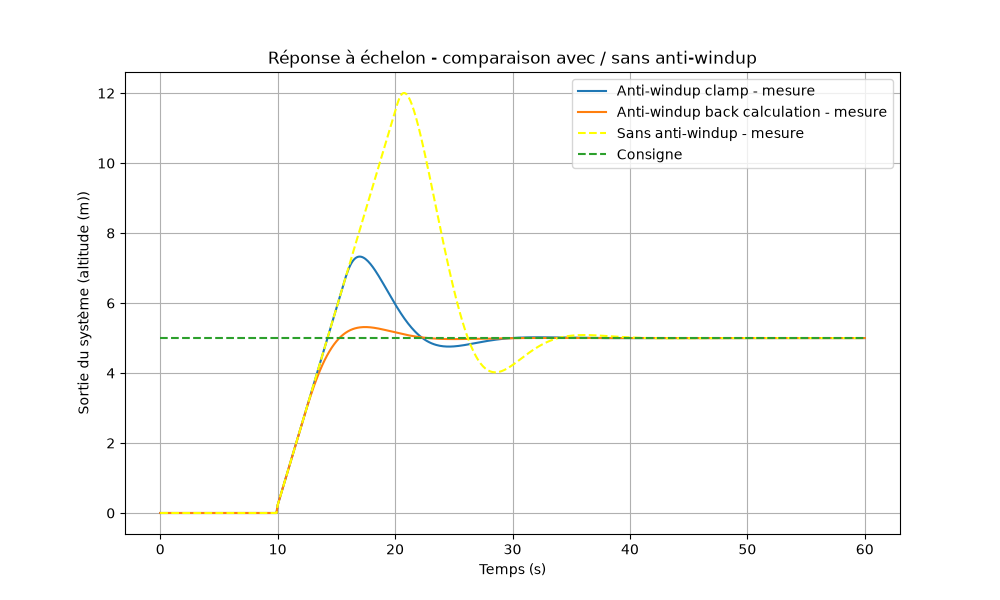
\includegraphics[width=\textwidth]{images/anti_windup_altitude.png}
    \caption{Altitude du drone en avec différents anti-windups avec la retenue}
    \label{fig:anti_windup_altitude_retenue}
\end{figure}

\begin{figure}
    \centering
    
\includegraphics[width=\textwidth]{images/anti_windup_altitude_sans_retenue.png}
    \caption{Altitude du drone en avec différents anti-windups sans la retenue}
    \label{fig:anti_windup_altitude_sans_retenue}
\end{figure}

\begin{figure}
    \centering
    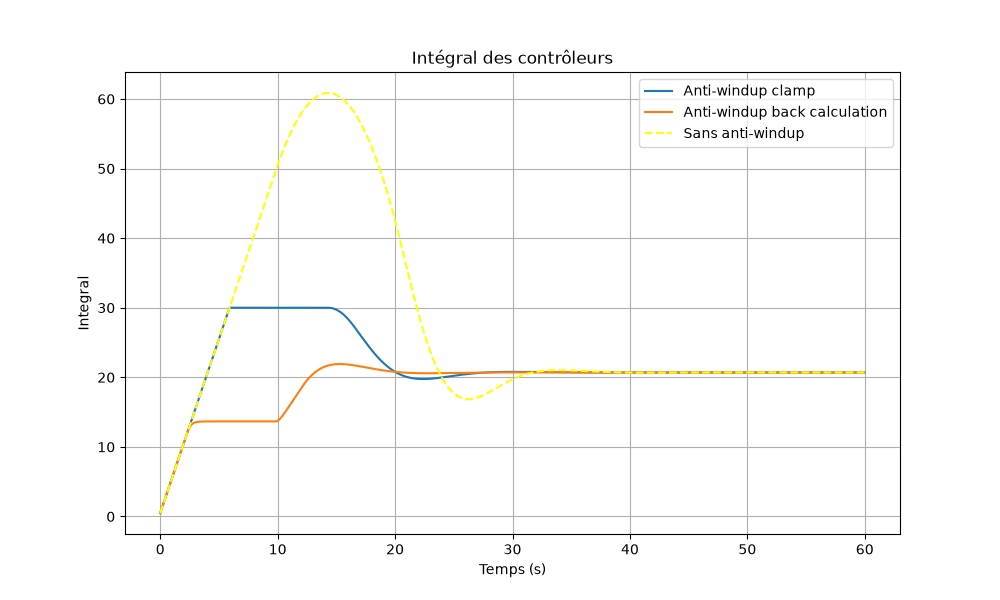
\includegraphics[width=\textwidth]{images/anti_windup_integral.png}
    \caption{Intégrale des différents anti-windups avec la retenue}
    \label{fig:anti_windup_integral_retenue}
\end{figure}

\begin{figure}
    \centering
    
\includegraphics[width=\textwidth]{images/anti_windup_integral_sans_retenue.png}
    \caption{Intégrale des différents anti-windups sans la retenue}
    \label{fig:anti_windup_integral_sans_retenue}
\end{figure}

\begin{figure}
    \centering
    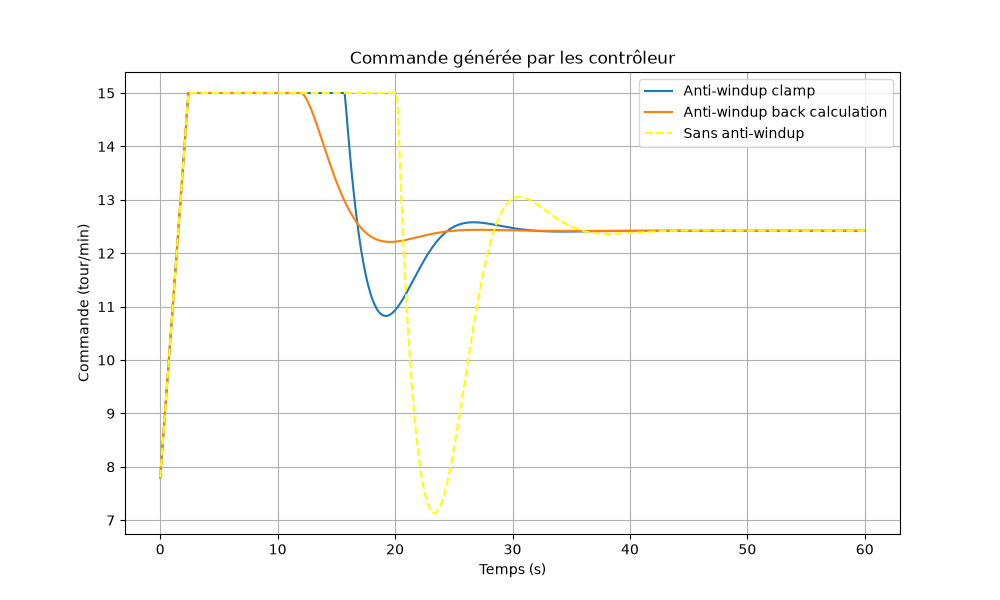
\includegraphics[width=\textwidth]{images/anti_windup_blade.png}
    \caption{Vitesse de rotation des hélices avec différents anti-windups avec retenue}
    \label{fig:anti_windup_blade_retenue}
\end{figure}

\begin{figure}
    \centering
    
\includegraphics[width=\textwidth]{images/anti_windup_blade_sans_retenue.png}
    \caption{Vitesse de rotation des hélices avec différents anti-windups sans retenue}
    \label{fig:anti_windup_blade_sans_retenue}
\end{figure}

\FloatBarrier


\newpage